\documentclass[../5RO17_TP1.tex]{subfiles}

\begin{document}
\subsection{Question 3}

\subsubsection{Direct Linear Transformation}
\noindent À partir de la définition de l'Homographie, l'application de la Direct Linear Transofmration (\textbf{DLT}) donne l'équation suivante :
\begin{equation}
    \underbrace{
        \begin{bmatrix}
            -x_{1_{1}} & -y_{1_{1}} & -1 & 0 & 0 & 0 & x_{2_{1}} x_{1_{1}} & x_{2_{1}} y_{1_{1}} & x_{2_{1}}\\
            0 & 0 & 0 & -x_{1_{1}} & -y_{1_{1}} & -1 & y_{2_{1}} x_{1_{1}} & y_{2_{1}} y_{1_{1}} & y_{2_{1}}\\
            & & & & \vdots\\
            -x_{1_{i}} & -y_{1_{i}} & -1 & 0 & 0 & 0 & x_{2_{i}} x_{1_{i}} & x_{2_{i}} y_{1_{i}} & x_{2_{i}}\\
            0 & 0 & 0 & -x_{1_{i}} & -y_{1_{i}} & -1 & y_{2_{i}} x_{1_{i}} & y_{2_{i}} y_{1_{i}} & y_{2_{i}}\\
            & & & & \vdots\\
            -x_{1_{N}} & -y_{1_{N}} & -1 & 0 & 0 & 0 & x_{2_{N}} x_{1_{N}} & x_{2_{N}} y_{1_{1}} & x_{2_{N}}\\
            0 & 0 & 0 & -x_{1_{N}} & -y_{1_{N}} & -1 & y_{2_{N}} x_{1_{N}} & y_{2_{N}} y_{1_{1}} & y_{2_{N}}\\
        \end{bmatrix}
    }_{\mathbf{A}}
    \underbrace{
        \begin{bmatrix}
            a_{11}\\ a_{12}\\ t_{x}\\ a_{21}\\ a_{22}\\ t_{y}\\ v_{1}\\ v_{2}\\ 1
        \end{bmatrix}
    }_{\mathbf{h}}
    =
    \begin{bmatrix}
        0\\ 0\\ 0\\ 0\\ 0\\ 0\\ 0\\ 0\\ 0\\
    \end{bmatrix}
\end{equation}
Cet équation peut être résolu à l'aide du méthode de Singular Value Decomposition (\textbf{SVD}):
\begin{equation}
    \underbrace{\mathbf{A}}_{2N\times9}
    =
    \underbrace{\mathbf{U}}_{2N\times9} \underbrace{\mathbf{S}}_{9\times9} \underbrace{\mathbf{V}}_{9\times9}
    \qquad
    \text{avec}
    \quad
    \begin{cases}
        \mathbf{U}^{\intercal}\mathbf{U} = \mathbf{I}_{9}\\
        \mathbf{V}^{\intercal}\mathbf{V} = \mathbf{I}_{9}\\
    \end{cases}
\end{equation}
Où $\mathbf{h}$ est donne par la dernière ligne de la matrice $\mathbf{V}$ avec les plus petits valeurs propres.

\subsubsection{Normalisation}
\noindent L'approche \textbf{DLT} permet algebriquement de trouver l'homographie necessaire pour récadre une image avec une erreur proporcionnelle à la taille de l'image. À fin de miniser l'influence de l'erreur sur les calcules une normalisation de l'image pourrait être applique.\\

\noindent La normalisation peut être fait avec la transformation suivant:
\begin{equation}
    \mathbf{T}
    =
    \begin{bmatrix}
        \frac{2}{w} & 0 & -1\\
        0 & \frac{2}{h} & -1\\
        0 & 0 & 1\\
    \end{bmatrix}
    \qquad
    \text{où}
    \quad
    \begin{cases}
        w & \text{width de l'image}\\
        h & \text{height de l'image}\\
    \end{cases}
\end{equation}
\noindent Cette transformation resize l'image pour que elle ait taille 2 par 2 et depuis change l'origine de l'image pour le centre du carré.\\

\noindent L'utilisation de cette méthode se fait comme explique ci-dessus:
\begin{enumerate}
    \item application de la normalisation sur les coordonnes:
    \begin{equation}
        \widetilde{\mathbf{x}}_{1_{i}} = \mathbf{T} \mathbf{x}_{1_{i}}
        \qquad
        \widetilde{\mathbf{x}}_{2_{i}} = \mathbf{T} \mathbf{x}_{2_{i}}
    \end{equation}
    \item application du méthode \textbf{DLT} avec les coordonnées normalisées
    \item application de la de-normalisation sur les coordonnes:
    \begin{equation}
        \mathbf{H} = \mathbf{T}^{-1} \widetilde{\mathbf{H}} \mathbf{T}
    \end{equation}
\end{enumerate}
\begin{remark}
    Aucune changement est necessaire pour l'algorithme \textbf{DLT}.
\end{remark}

\subsubsection{Résultats}
\noindent Après cette calcule théorique, ses expressions ont été implementées en Python et l'image suivante a été obtenu:
\begin{figure}[H]
    \centering
    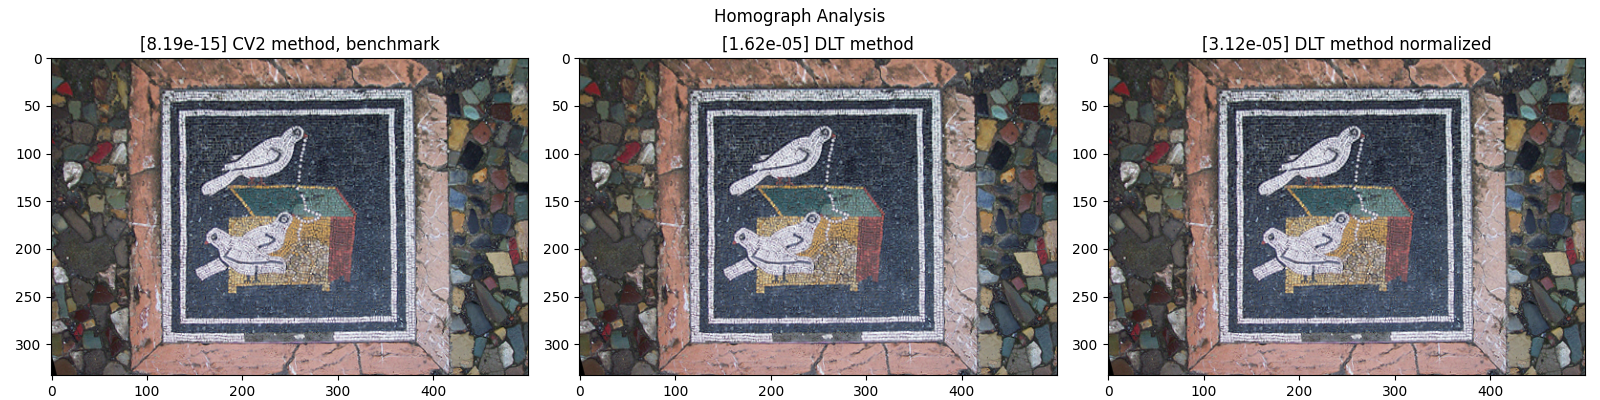
\includegraphics[width = \linewidth]{../images/homography.png}
    \caption{Application de l'Homographie}
    \label{fig:homography}
\end{figure}
\noindent L'image plus à gauche présent le résultat obtenu avec la fonction \texttt{cv2.homography()}, l'image au mieu présent le résultat obtenu avec le méthode \textbf{DLT} sans normalisation et l'image plus à la droite présent le résultat obtenu avec le méthode \textbf{DLT} avec normalisation.

\subsubsection{Erreur}
\noindent Sur le titre de chaque image, l'erreur est présente pour que les différentes méthodes puissent être comparées. Dans ce cas, l'indice de confiance choisi a été \textbf{l'Erreur de Reprojection}, qui permet de mesurer la proximité des points projetés par l'homographie par rapport aux points de l'image originale. Ainsi, plus l'erreur de reprojection est petite, meilleure est la correspondance entre les points de la source et les points corrigés.\\

\noindent L'Erreur de Reprojection est calculée avec l'équation ci-dessous:
\begin{equation}
    \text{ER} = \sqrt{\sum^{n}_{i=0} ||\bf{p}_{d_{i}} - \bf{p}_{s_{i}}||}
\end{equation}
\noindent Avec l'implémentation suivante en Python:
\begin{scriptsize}\mycode
	\begin{lstlisting}[language=Python]
def get_reprojection_error(homograph: np.array, src_pts: np.array, dst_pts: np.array) -> float:
    """
    Return reprojection error of homograph.

    Note: how closely the projected points via the homograph match the actual points in the image.

    Args:
        homograph (np.array) : homograph matrix.
        src_pts (np.array) : source image points.
        dst_pts (np.array) : destination image points.
    """
    projected_pts = cv2.perspectiveTransform(src_pts.reshape(-1, 1, 2), homograph).reshape(-1, 2)
    error = np.sqrt(np.sum((projected_pts - dst_pts) ** 2, axis=1))

    return np.mean(error)
	\end{lstlisting}
\end{scriptsize}

\subsubsection{Analyse}
\noindent Il est notable qu'avec cette erreur, la méthode normalisée entraîne une erreur plus importante, environ le double, par rapport à la méthode non normalisée. Cela pourrait être causé par la taille de l'image, qui n'était pas très élevée, et le fait que la dénormalisation nécessite une inversion de matrice, ce qui peut accumuler des erreurs numériques significatives.\\

\noindent Le résultat obtenu avec OpenCV est ajouté à l'image ci-dessus comme référence d'un résultat idéal, et comme attendu, c'est la méthode qui présente la plus petite erreur parmi les trois méthodes implémentées, montrant l'optimisation des fonctions utilisées par OpenCV.\\

\noindent Il est curieux que la normalisation, dans ce cas, présente un résultat marginalement moins efficace que la version non normalisée. Cela dit, cet effet peut être dû au fait que la taille de l'image originale n'est pas très grande et que l'erreur de l'homographie est moins significative que l'erreur numérique introduite par l'inversion de matrices nécessaire à la normalisation.
\end{document}
